$subject$=Физические основы компьютерных \\ и сетевых технологий
$teacher$=Лекции Герта А. В.
$date$=24.02.2025

\section{Лекция 3. Сила Ампера. Явление электромагнитной индукции}

\subsection{Сила Ампера}

Вектор магнитной индукции характеризует силовое действие магнитного поля на движущиеся заряды. 
Сила, действующая на движущийся точечный зарядв магнитном поле, равна $\vec{F}_{\text{Л (М)}} = q [\vec{v}, \vec{B}]$
и называется магнитной составляющей силы Лоренца

Направление магнитной составляющей силы Лоренца зависит от знака заряженной частицы

Магнитная составляющая силы Лоренца всегда направлена перпендикулярно скорости, поэтому не совершает работы и не изменяет величину скорости заряженной частицы

\begin{wrapfigure}{r}{0pt}
    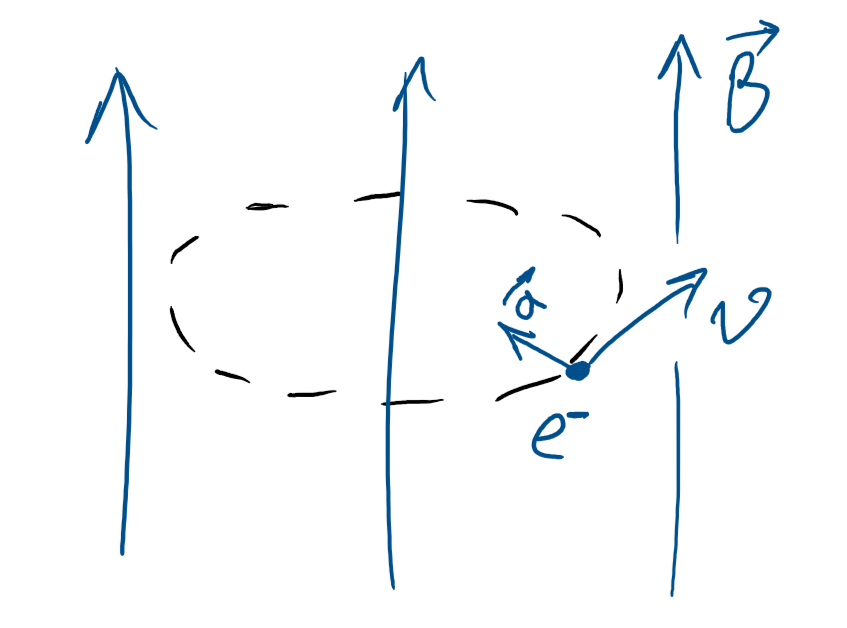
\includegraphics[width=6.2cm]{physics2/images/physics2_2025_02_24_1}
\end{wrapfigure}

\Ex Частица влетает перпендикулярно силовым линиям магнитного поля: $\vec{v} \perp \vec{B}$

Скорость частицы и действующая на нее сила все время лежат в плоскости, перпендикулярной к силовым линиям магнитного поля. 
Траекторией движения частицы будет окружность радиуса $R$, лежащая в этой плоскости. 
Условием движения по окружности является $q v B = m\frac{v^2}{R}$, из этого $R = \frac{mv}{qB}$


\Ex Частица влетает под углом $\alpha$ к силовым линиям магнитного поля

Составляющая скорости, направленная вдоль силовых линий магнитного поля, не будет изменяется, 
а в плоскости, перпендикулярной силовым линиям, частица движется по окружности. Траектория движения 
представляет собой винтовую линию

\Mem Сила Лоренца - полная сила, действующая на заряд: $\vec{F}_\text{Л} = q\vec{E} + q[\vec{v}, \vec{B}]$

Разделение полной силы Лоренца на электрическую и магнитную зависит от выбора системы отсчета

\Def Сила Ампера - сила, действующая под действием магнитного поля на заряды проводника, создающие электрический ток

Пусть электрический ток в объеме $dV$ элемента тока длиной $dl$ и площадью сечения $S$ образован заряженными частицами с зарядом
$q$, движущимися со средней скоростью $v$ вдоль элемента тока: 

\[d\vec{F}_A = [\vec{j}, \vec{B}] dV\]

\[d\vec{F}_A = I [d\vec{l}, \vec{B}]\]

Направление силы Ампера можно определить с помощью правила левой руки: если ладонь левой руки расположить так,
чтобы в нее входил вектор индукции магнитного поля, а четыре вытянутых - пальца по направлению тока, то отогнутый
на $90^\circ$ большой палец покажет направление силы Ампера

Для изучения свойств магнитного поля используется замкнутый плоский контур с током (рамка с током). Форма контура
не имеет значения, а его размеры должны быть малы по сравнению с расстоянием до источников магнитного поля.
Контур с током принято характеризовать магнитным моментом: $\vec{p}_m = I S \vec{n}$, где $I$ - сила тока, $S$ - площадь,
ограниченная контуром, $\vec{n}$ - нормаль, образующая с направлением тока правовинтовую систему

На контур с током действует сила Ампера $d\vec{F}_A = I[d\vec{l}, \vec{B}] \Longrightarrow \vec{F}_A = I \oint [d\vec{l}, \vec{B}]$

Если поле однородно, то $\vec{F}_A = I \oint [d\vec{l}, \vec{B}] = I [\oint d\vec{l}, \vec{B}] = 0$

Если поле неоднородно, то $\vec{F} = p_m \frac{\partial \vec{B}}{\partial n}$

\begin{wrapfigure}{r}{0pt}
    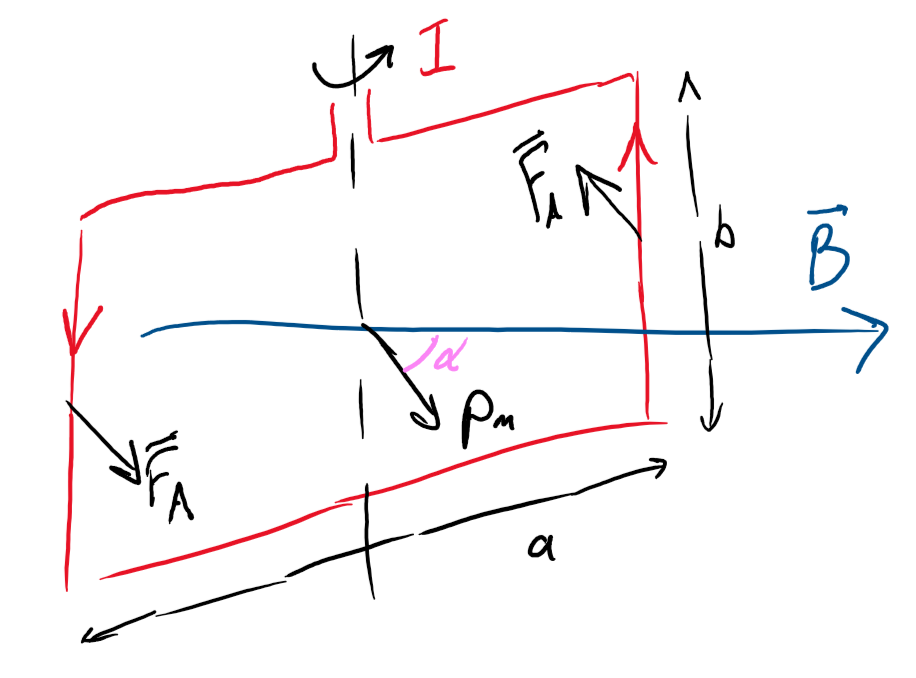
\includegraphics[width=7cm]{physics2/images/physics2_2025_02_24_2}
\end{wrapfigure}

\Ex Рассмотрим случай поведения прямоугольного контура с током в однородном магнитном поле. 
Предположим, что рамка имеет возможность вращаться вокруг оси, проходящей через середины ее
сторон длиной $a$ и перпендикулярной к силовым линиям магнитного поля.

Силы Ампера, действующие на стороны $a$ рамки, направлены вдоль оси вращения, 
поэтому действие этих сил сводится только к деформации контура (сжатию или растяжению).
Силы Ампера, действующие на стороны $b$ рамки, создают вращающий момент и равны $F_A = IBb$.

Тогда момент сил равен $M = F a \sin \alpha = I B S \sin \alpha = p_m B \sin \alpha \Longrightarrow \vec{M} = [\vec{p}_m, \vec{B}]$

\begin{wrapfigure}{r}{0pt}
    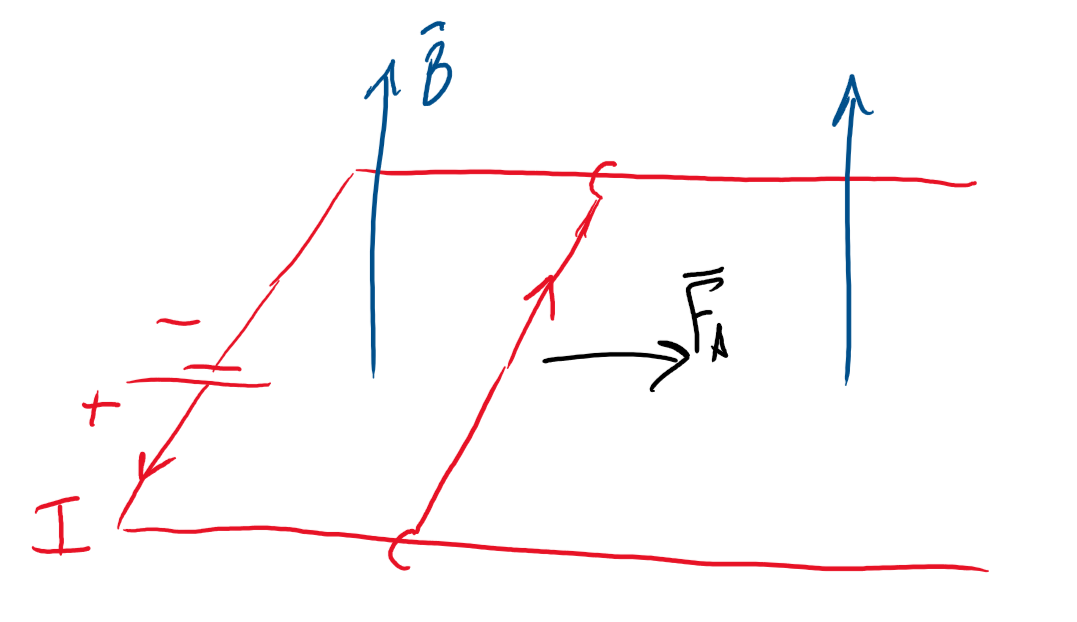
\includegraphics[width=7cm]{physics2/images/physics2_2025_02_24_3}
\end{wrapfigure}

\Ex Рассмотрим проводник в форме буквы \enquote{П} и двигающийся по нему другой проводник. 
По контуру, находящемуся в магнитном поле, течет ток, значит подвижный проводник будет двигаться влево, 
увеличивая площадь, охватываемого контуром. 

Работа сил магнитного поля по перемещению подвижного проводника будет равна:

$dA = d\vec{F} \cdot d\vec{r} = I [d\vec{l}, \vec{B}] \cdot d\vec{r} = Id\Phi$

$A = \int_1^2 Id\Phi$


\subsection{Явление электромагнитной индукции. Закон Фарадея. Правило Лоренца}

\begin{wrapfigure}{r}{0pt}
    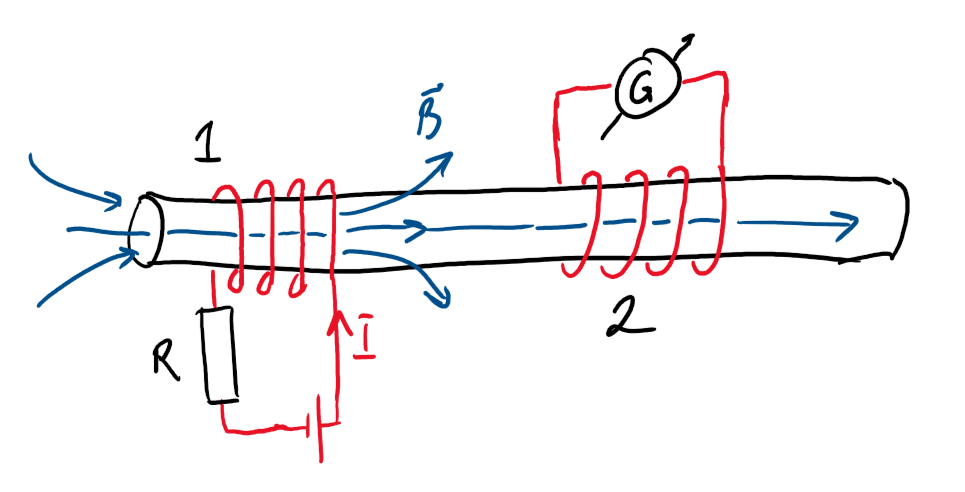
\includegraphics[width=6.2cm]{physics2/images/physics2_2025_02_24_4}
\end{wrapfigure}

В цепи первой катушки течет постоянный ток $I_1$, в цепи второй ток отсутствует. 
Если катушку 1 приближать к 2, в последней возникнет ток $I_2$, который Фарадей назвал индукционным током. 
При удалении катушки 1 от 2 ток $I_2$ тоже появляется, но имеет противоположное направление.

Катушку 1 можно заменить длинным полосовым магнитом. При перемещении магнита вдоль оси катушки 2, тоже обнаружится возникновение в ней 
индукционного тока.

Явление электромагнитной индукции заключается в возникновении электрического тока в замкнутом проводящем
контуре при изменении магнитного потока, охватываемого этим контуром. 

\begin{MyTheorem}
    Закон Фарадея: ЭДС индукции в контуре пропорциональна скорости изменения магнитного потока сквозь площадь, 
    ограниченную контуром:

    \[\varepsilon = - \frac{d\Phi}{dt}\]
\end{MyTheorem}

\begin{MyTheorem}
    Правило Ленца: индукционный ток всегда направлен так, что его магнитное поле противодействует причине, вызвавшей его появление
\end{MyTheorem}

Самоиндукцией называется явление возникновение ЭДС индукции в электрической цепи вследствие
изменения электрического тока в этой же цепи.

Заметим, что $B \sim I$ и $\Phi \sim B$ (в отсутствии ферромагнетиков). Тогда $\Phi \sim I$ или же $\Phi = LI$

Коэффициент пропорциональности $L$ называется индуктивностью контура. Индуктивность контура зависит от его размеров
и формы, магнитных свойств среды

При изменении силы тока в контуре возникает ЭДС самоиндукции $\varepsilon_s = -\frac{d\Phi}{dt} = -\frac{d}{dt}(LI) = -L\frac{dI}{dt} - I\frac{dL}{dt}$

\clearpage
